
\subsection{1. 前言}

\subsubsection{后缀数组和后缀树}

\begin{QUOTE}{}{}
在字符串处理当中,后缀树和后缀数组都是非常有力的工具。其实后缀数组是后缀树的一个非常精巧的替代品,它比后缀树容易编程实现,能够实现后缀树的很多功能而时间复杂度也不太逊色,并且,它比后缀树所占用的空间小很多。可以说,在信息学竞赛中后缀数组比后缀树要更为实用。——百度百科
\end{QUOTE}

\subsubsection{各种定义}

\texttt{子串}: 就是子串 [捂脸]

\texttt{后缀}: 就是从 $i$ 这个位置开始到该字符串的末尾的一个子串

\texttt{字符串大小}: $a$ 和 $b$ 这两个串,从头开始逐个字符按照 ASSIC 码进行比较

\texttt{后缀数组}: $sa[i]$ 代表该字符串的 $len$ 个后缀中,排名为 $i$ 的后缀是第 $sa[i]$ 个后缀

\texttt{名词数组}: $rank[i]$ 代表第 $i$ 个后缀排名为 $rank[i]$

\subsection{2. 一些构造方法}

\subsubsection{最简单的暴力}

把所有的后缀拆出来,然后 sort

思想较为简单,可自行尝试实现

\begin{cppcode}
#include <bits/stdc++.h>
using namespace std;

int rank[123], sa[123];

struct Str {
  string s;
  int wei;
  friend bool operator<(Str a1, Str a2) { return a1.s < a2.s; }
} k[123];

int main() {
  string s;
  cin >> s;
  int len = s.size() - 1;

  for (int i = 0; i <= len; i++) {
    k[i].wei = i;
    for (int j = i; j <= len; j++) k[i].s = k[i].s + s[j];
  }

  sort(k, k + len + 1);
  for (int i = 0; i <= len; i++) {
    rank[k[i].wei] = i;
    sa[i] = k[i].wei;
  }

  exit(0);
}
\end{cppcode}

\subsubsection{倍增}

这个就是一般人写后缀数组用的方法

复杂度是 $O(nlogn)$ 

前提是你要先会 \textbf{ 基数排序 }

假设我们有这样一个字符串 \texttt{aabaaaab}

然后我们把所有的后缀列举出来:

\begin{figure}[htbp]
\centering
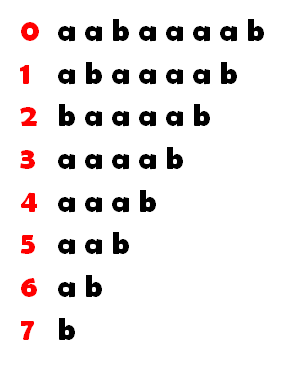
\includegraphics[width=0.7\textwidth]{docs/string/images/sa1.png} 

\end{figure}

然后用基数排序的方式,按照每个后缀的第一个字母进行排序,呈现这样子的效果:

\begin{figure}[htbp]
\centering
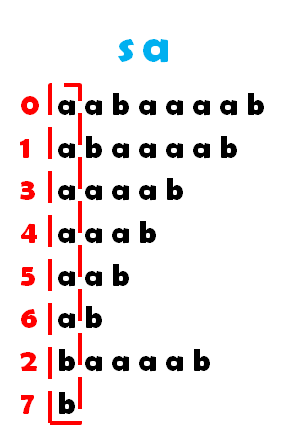
\includegraphics[width=0.7\textwidth]{docs/string/images/sa2.png} 

\end{figure}

接着我们以第二个字母为关键字,在首字母有序的基础上进行排序,这个时候,我们把首字母相同的后缀拿出来单看

对于每一组首字母相同的后缀,首字母是对排序没有影响的,所以可以直接按照第二个字母进行基数排序,同样,对于首字母不同的后缀,由于按照首字母排序时,他们的相对大小已经确定,当按照第二个字母排序时,不会出现 \texttt{原来 a>b,现在 b>a} 的现象,所以我们可以看成一直在做区域内的排序,这之后变成这样:

\begin{figure}[htbp]
\centering
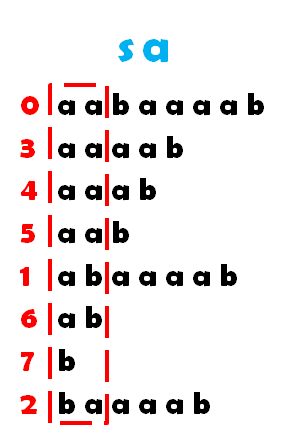
\includegraphics[width=0.7\textwidth]{docs/string/images/sa3.png} 

\end{figure}

第三字母同理........

这样子我们可以处理这个问题,可是复杂度还是没有到达一个我们可以接受的范围

所以我们引入 \textbf{ 倍增 }

当我们按照每个后缀的前 $2^k$ 个字母进行完排序后,那么我们把后缀的前 $2^{k+1}$ 看做前后两个 $2^k$, 这样我们就可以把这前后两个 $2^k$ 作为之前说的 \texttt{首字母} 和 \texttt{第二个字母} 了,然后进行上述过程,就可以在 $O(nlogn)$ 的复杂度内处理这个问题了

\begin{cppcode}
#include <bits/stdc++.h>
using namespace std;

int n;
int sa[150], x[150], c[150], y[150];
char a[150];

inline void SA() {
  int m = 128;
  for (int i = 0; i <= m; i++) c[i] = 0;
  for (int i = 1; i <= n; i++) c[x[i]]++;
  for (int i = 1; i <= m; i++) c[i] += c[i - 1];
  for (int i = n; i; i--) sa[c[x[i]]--] = i;

  for (int k = 1, p; k <= n; k <<= 1) {
    p = 0;
    for (int i = n; i > n - k; i--) y[++p] = i;
    for (int i = 1; i <= n; i++)
      if (sa[i] > k) y[++p] = sa[i] - k;

    for (int i = 0; i <= m; i++) c[i] = 0;
    for (int i = 1; i <= n; i++) c[x[i]]++;
    for (int i = 1; i <= m; i++) c[i] += c[i - 1];
    for (int i = n; i; i--) sa[c[x[y[i]]]--] = y[i];

    p = y[sa[1]] = 1;
    for (int i = 2, a, b; i <= n; i++) {
      a = sa[i] + k > n ? -1 : x[sa[i] + k];
      b = sa[i - 1] + k > n ? -1 : x[sa[i - 1] + k];
      y[sa[i]] = (x[sa[i]] == x[sa[i - 1]]) && (a == b) ? p : ++p;
    }
    swap(x, y);
    m = p;
  }
}

int main() {
  scanf("%s", a + 1);

  n = strlen(a + 1);
  for (int i = 1; i <= n; i++) x[i] = a[i];
  SA();

  for (int i = 1; i <= n; i++) printf("%d", sa[i]);
  exit(0);
}
\end{cppcode}

代码里 $x[i]$ 就是 $rank[i]$ 

$y[i]$ :假设 $y[i]=a\ ,\  y[i+1]=b$ 那么在原串中 从 $a+2^k$ 开始的 $2^k$ 个字符组成的子串 \textbf{ 小于等于 } 从 $b+2^k$ 开始的 $2^k$ 个字符组成的子串

最好理解这个代码时,每一步都结合这基数排序来考虑
